\begin{figure}
  \centerline{
    \setlength{\tabcolsep}{2.0pt}
  \begin{tabular}{cccc}
    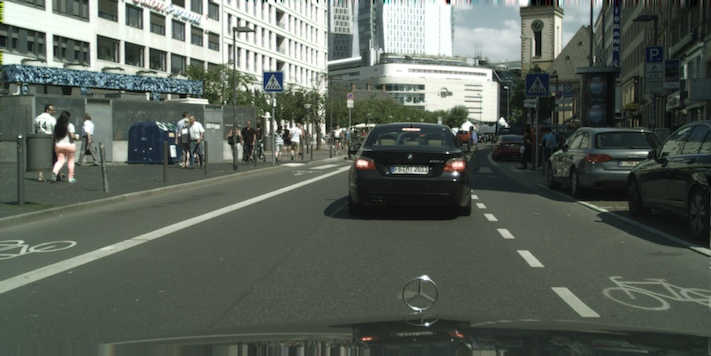
\includegraphics[width=\myw, height=\myh]{figs/gta2city_color/4_img.png} &
	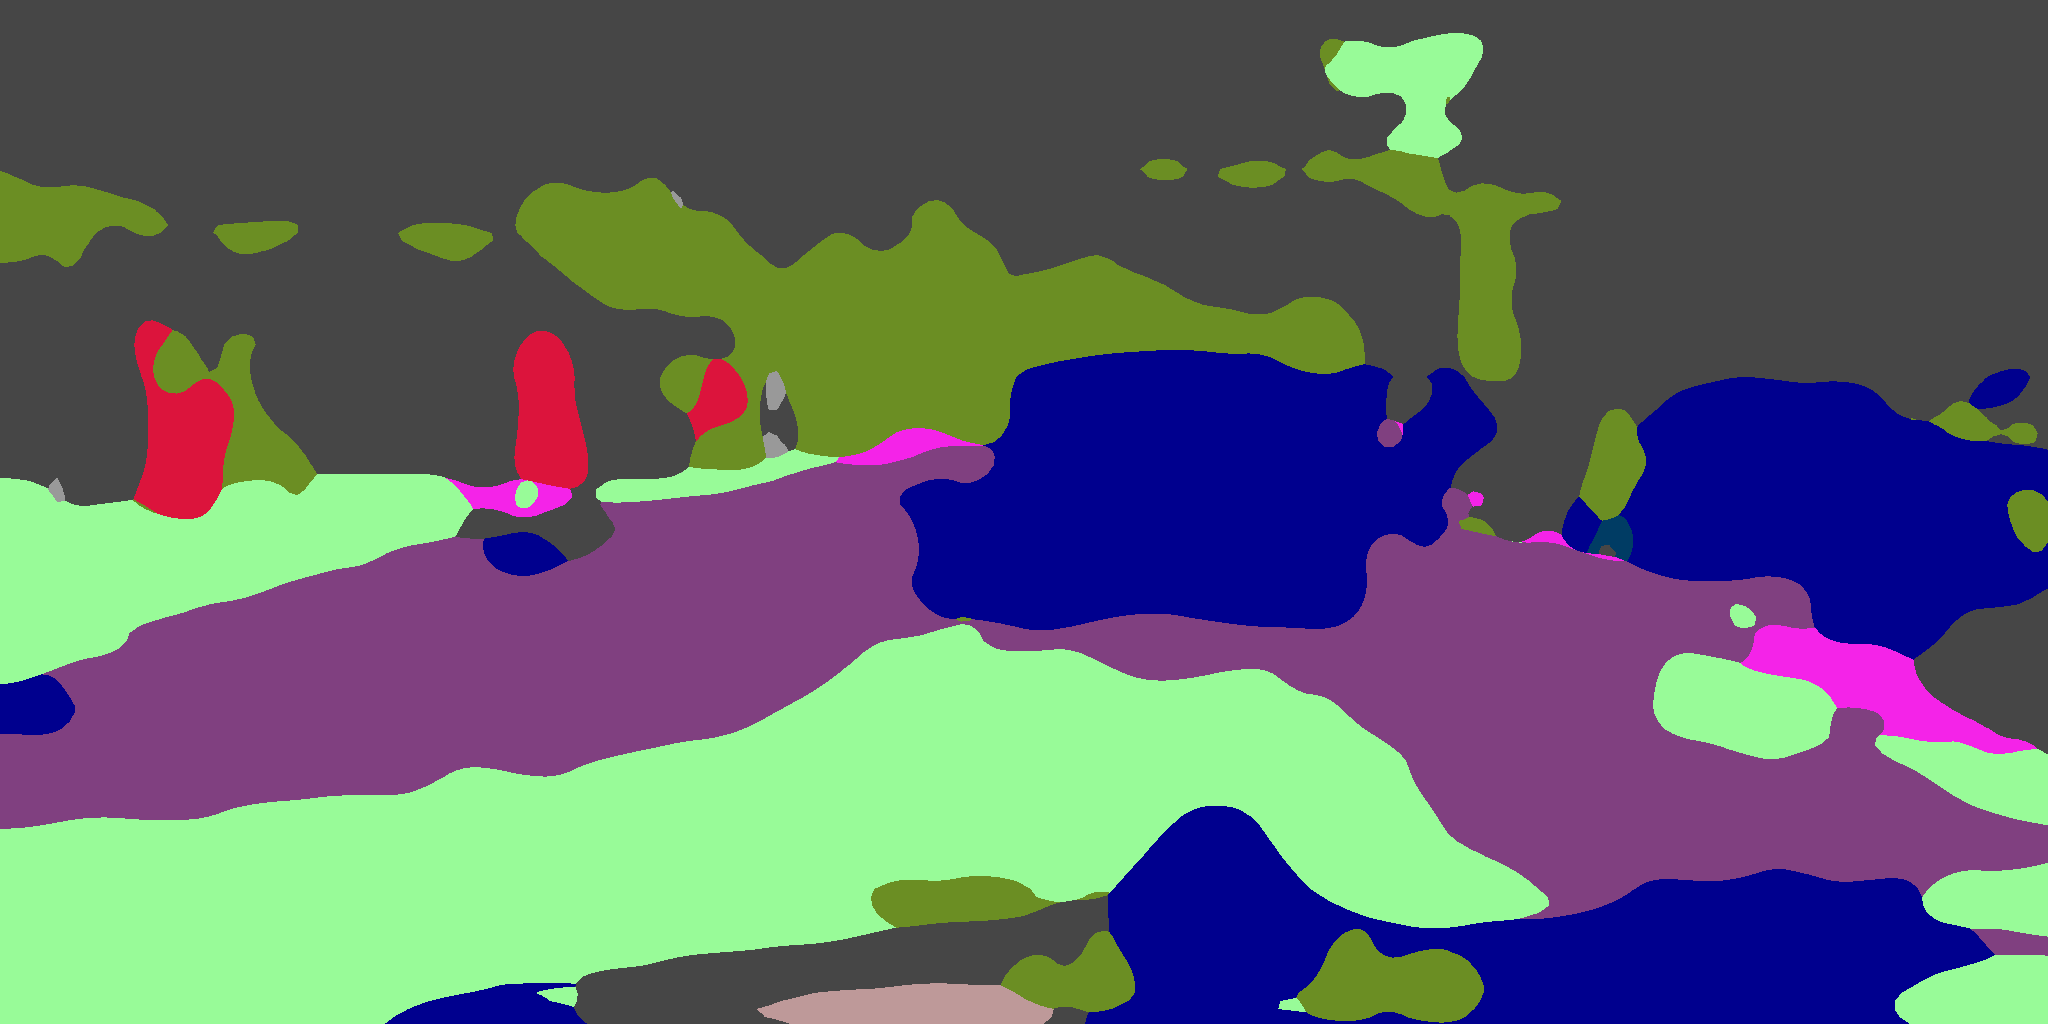
\includegraphics[width=\myw, height=\myh]{figs/gta2city_color/4_src.png} &
	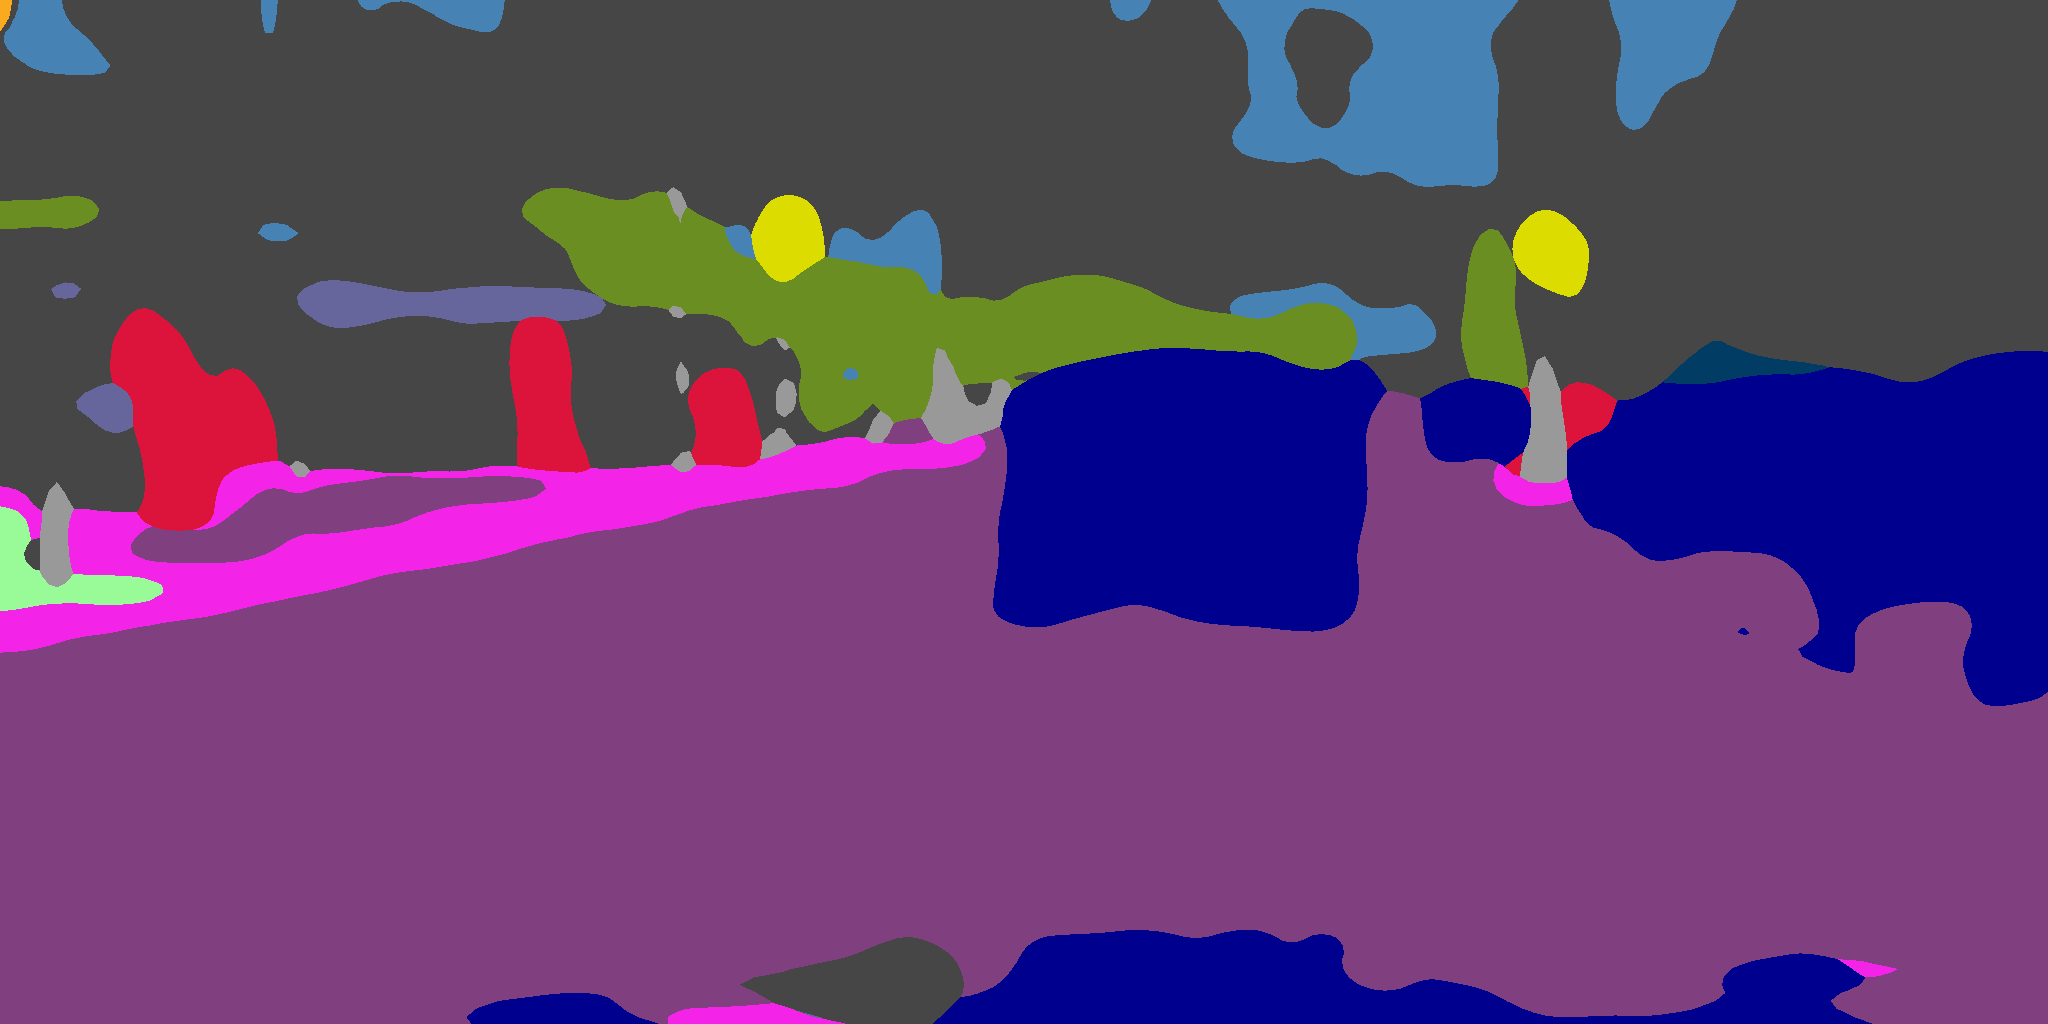
\includegraphics[width=\myw, height=\myh]{figs/gta2city_color/4_cycada.png} &
	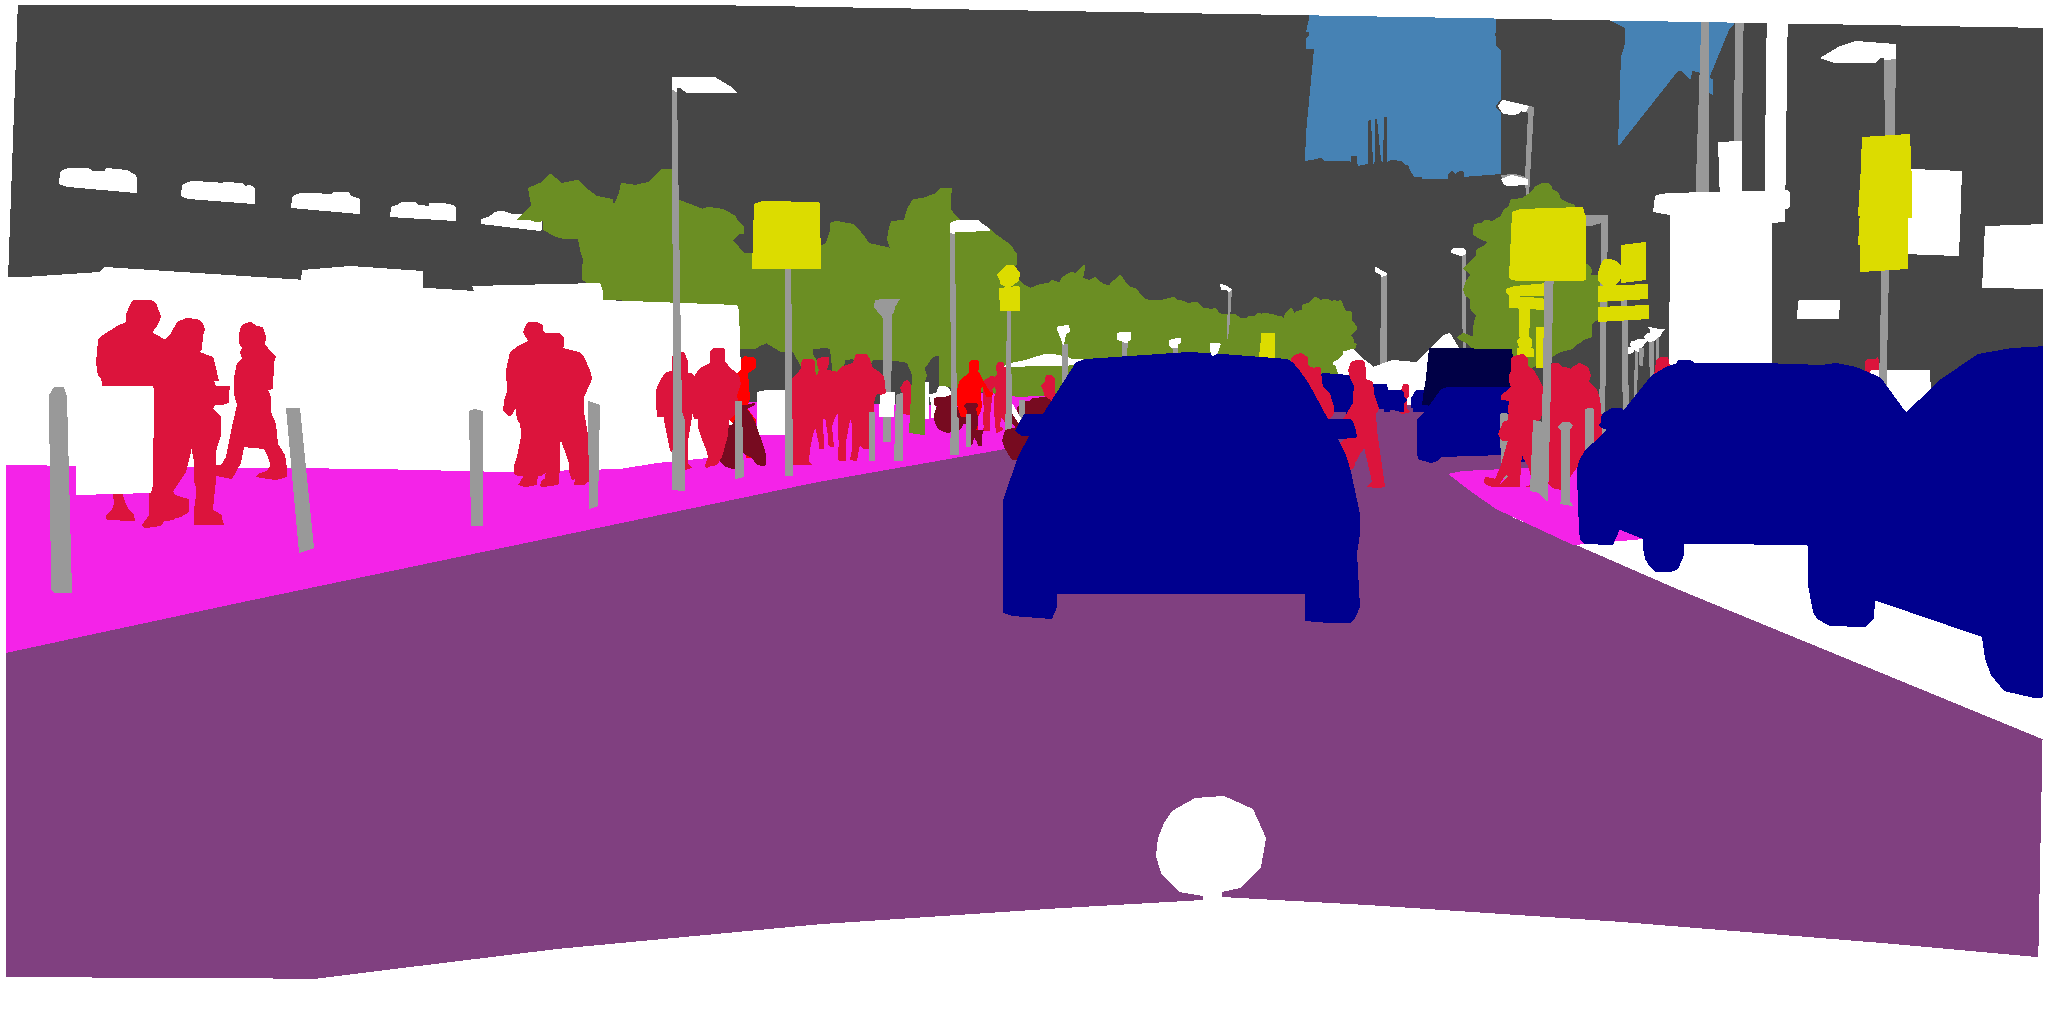
\includegraphics[width=\myw, height=\myh]{figs/gta2city_color/4_gt.png} 
   \\
   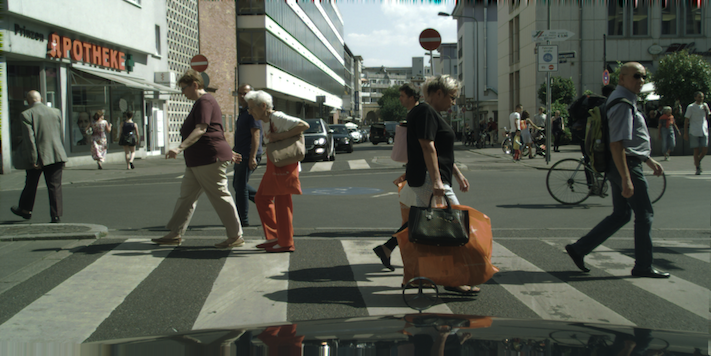
\includegraphics[width=\myw, height=\myh]{figs/gta2city_color/25_img.png} &
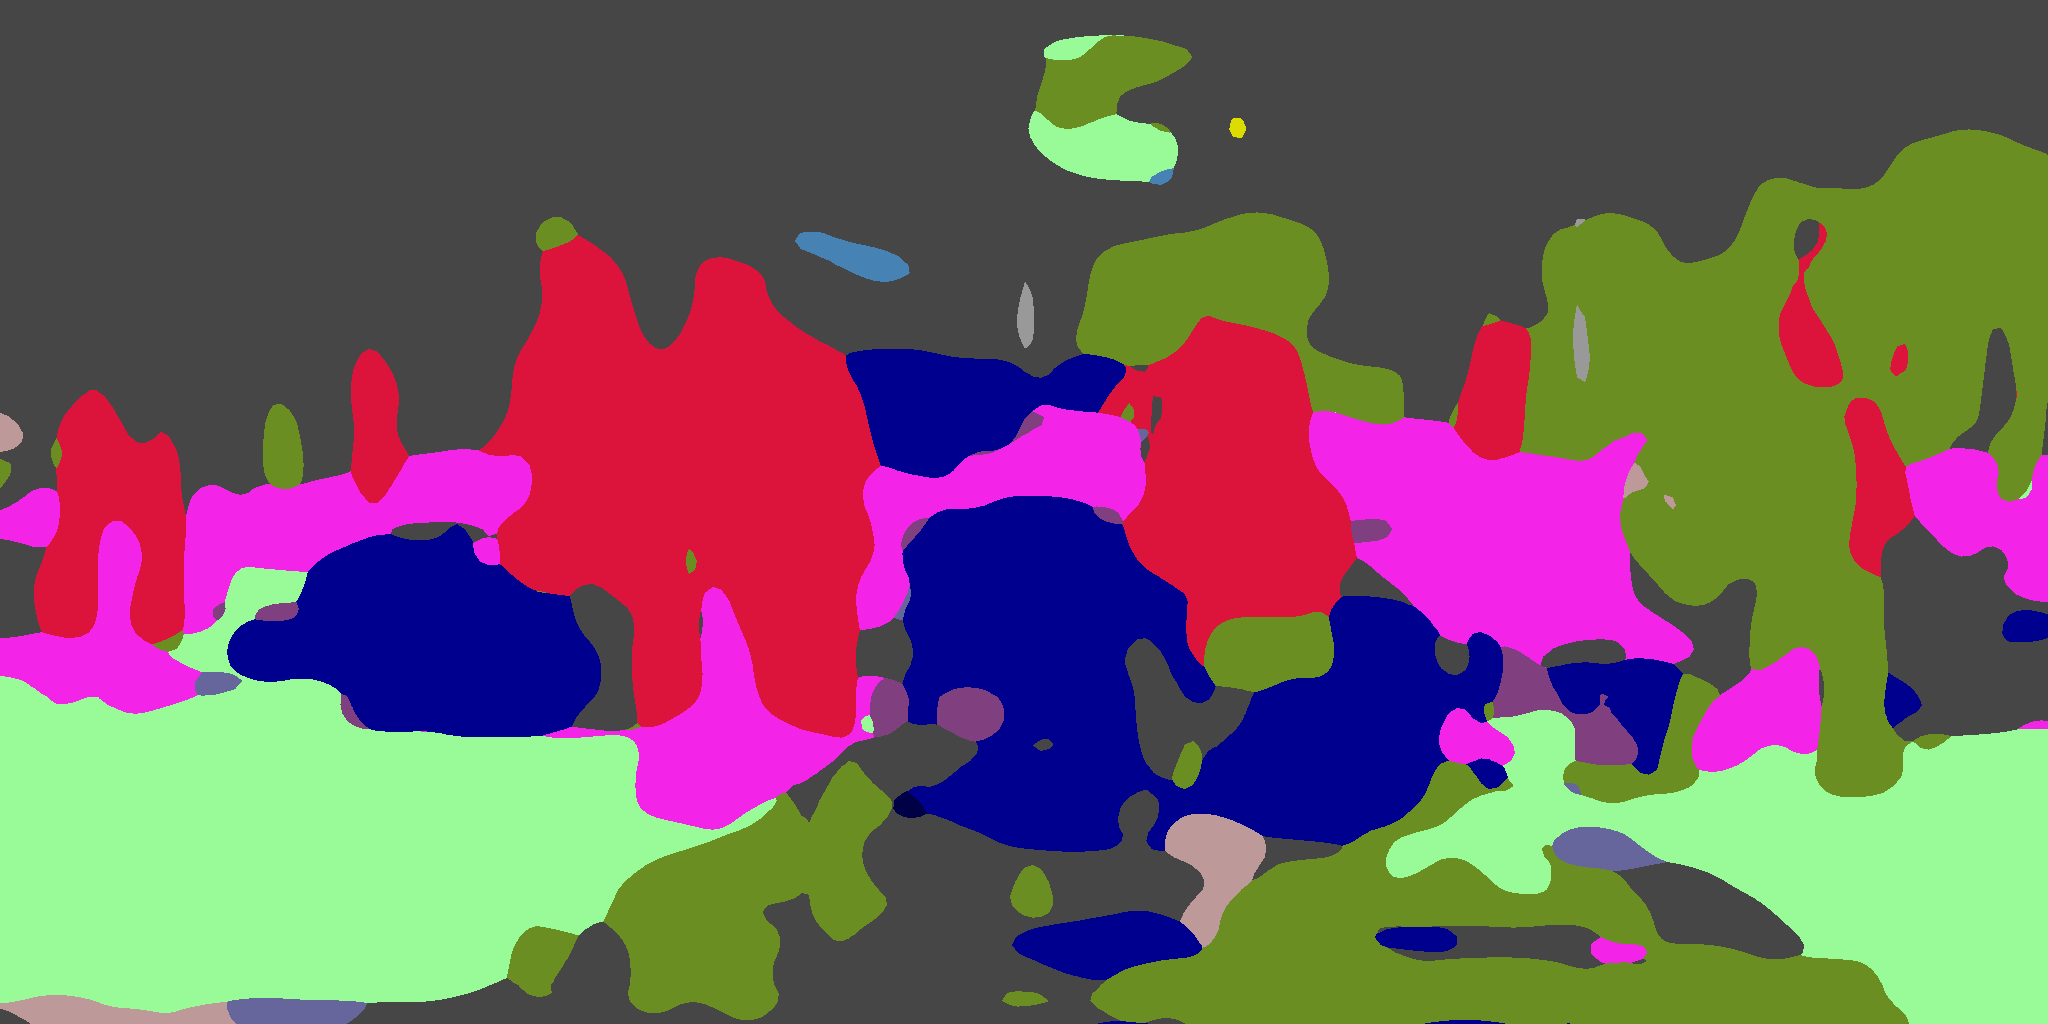
\includegraphics[width=\myw, height=\myh]{figs/gta2city_color/25_src.png} &
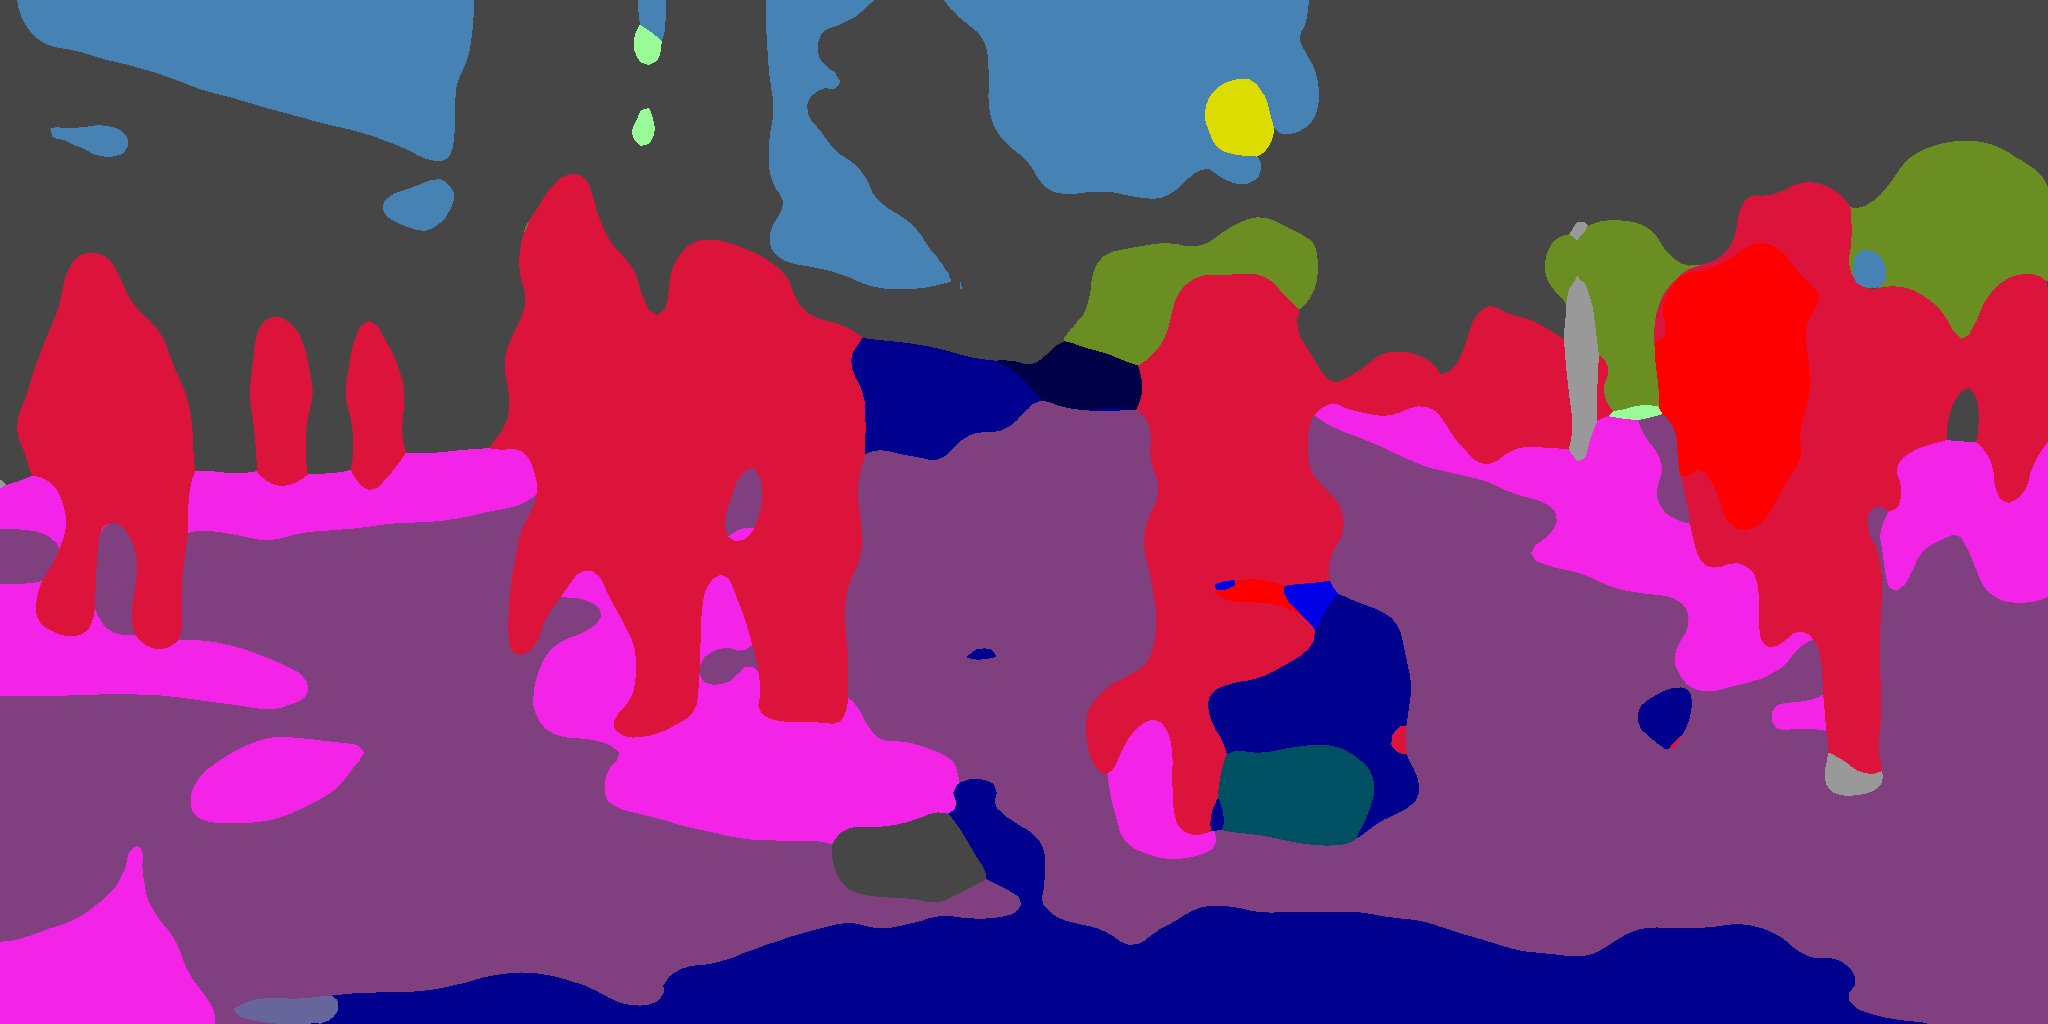
\includegraphics[width=\myw, height=\myh]{figs/gta2city_color/25_cycada.png} &
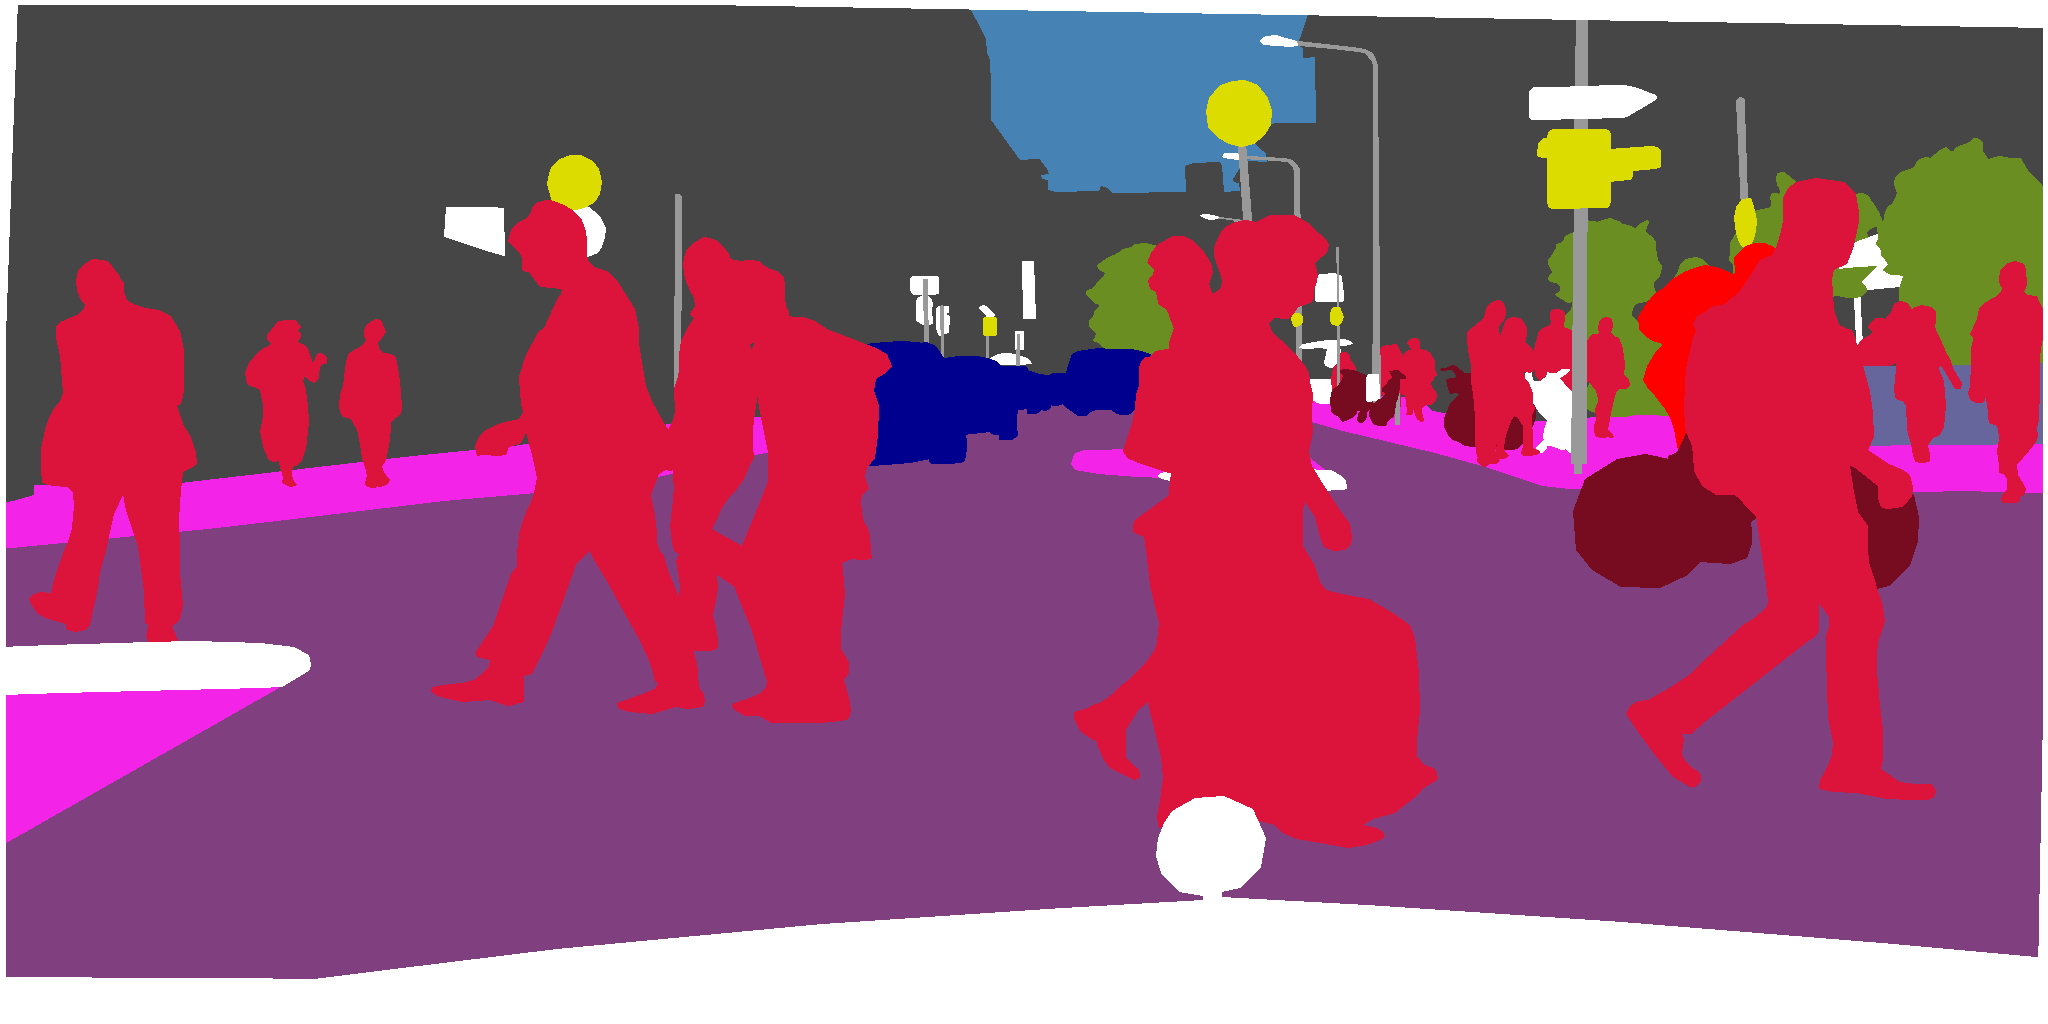
\includegraphics[width=\myw, height=\myh]{figs/gta2city_color/25_gt.png}
\\
   (a) Test Image & (b) Source Prediction & (c) CyCADA Prediction & (d) Ground Truth\\
  \end{tabular}
  }
  \caption{%\small 
  \textbf{GTA5 to CityScapes Semantic Segmentation.} Each test CityScapes image (a) along with the corresponding predictions from the source only model (b) and our CyCADA model (c) are shown and may be compared against the ground truth annotation (d). }
  \label{fig:gta-cityscapes-seg}
\end{figure}


